\documentclass[aspectratio=169, 10pt]{beamer}

% ============================================================
% THEME & COLORS - Madrid Standard (Matching Original Report)
% ============================================================
\usetheme{Madrid}
\usecolortheme{default}
\setbeamertemplate{navigation symbols}{}
\setbeamertemplate{blocks}[rounded][shadow=true]

% Custom Colors (Consistent with Original)
\definecolor{espblue}{RGB}{0, 100, 148}
\definecolor{espgold}{RGB}{255, 196, 37}
\definecolor{codegreen}{RGB}{40, 167, 69}
\definecolor{codeorange}{RGB}{253, 126, 20}
\definecolor{codepurple}{RGB}{111, 66, 193}
\definecolor{codered}{RGB}{220, 53, 69}
\definecolor{darkbg}{RGB}{40, 44, 52}
\definecolor{lightgray}{RGB}{248, 249, 250}
\definecolor{appred}{RGB}{239, 154, 154}
\definecolor{appblue}{RGB}{144, 202, 249}
\definecolor{apppurple}{RGB}{206, 147, 216}
\definecolor{osgreen}{RGB}{165, 214, 167}
\definecolor{kernelblue}{RGB}{100, 181, 246}
\definecolor{hwgray}{RGB}{189, 189, 189}

% ============================================================
% PACKAGES
% ============================================================
\usepackage{tikz}
\usetikzlibrary{shapes.geometric, shapes.symbols, shapes.misc, arrows.meta, positioning, calc, fit, backgrounds, decorations.pathreplacing, shadows, patterns, chains, matrix}
\usepackage{listings}
\usepackage{xcolor}
\usepackage{amsmath, amssymb}
\usepackage{booktabs}
\usepackage{graphicx}

% ============================================================
% CODE LISTING STYLES
% ============================================================
\lstdefinestyle{cstyle}{
    language=C,
    basicstyle=\ttfamily\tiny,
    keywordstyle=\color{codepurple}\bfseries,
    stringstyle=\color{codegreen},
    commentstyle=\color{gray}\itshape,
    numberstyle=\tiny\color{gray},
    breaklines=true,
    showstringspaces=false,
    tabsize=2,
    frame=single,
    backgroundcolor=\color{lightgray},
    morekeywords={uint32_t, int32_t, size_t, Elf32_Phdr, esp_err_t, bool, ssize_t},
    escapeinside={(*@}{@*)},
}

\lstnewenvironment{ccode}[1][]
{\lstset{style=cstyle,title={\tiny #1}}}
{}

% ============================================================
% TikZ STYLES
% ============================================================
\tikzset{
    layerbox/.style={draw, rectangle, minimum width=2.5cm, minimum height=0.7cm, font=\scriptsize, align=center, thick},
    appbox/.style={layerbox, fill=appred!60},
    osbox/.style={layerbox, fill=osgreen!60},
    kernelbox/.style={layerbox, fill=kernelblue!60},
    hwbox/.style={layerbox, fill=hwgray!60},
    shimbox/.style={layerbox, fill=espgold!40},
    guestbox/.style={layerbox, fill=codegreen!30, draw=codegreen!70!black},
    component/.style={draw, rectangle, rounded corners=2pt, minimum width=2.2cm, minimum height=0.6cm, font=\scriptsize, align=center},
    kernel/.style={component, fill=espblue!20, draw=espblue},
    guest/.style={component, fill=codegreen!20, draw=codegreen!70!black},
    hardware/.style={component, fill=gray!30, draw=gray!60},
    shim/.style={component, fill=espgold!30, draw=espgold!70!black},
    danger/.style={component, fill=codered!20, draw=codered},
    dataarrow/.style={-{Stealth[length=2mm]}, thick, draw=espblue},
    callarrow/.style={-{Stealth[length=2mm]}, thick, draw=codegreen!70!black},
    annotation/.style={font=\tiny\itshape, text=gray},
}

% ============================================================
% METADATA
% ============================================================
\title[TLCL: Recent Improvements]{ESP32 TLCL: Recent Improvements}
\subtitle{Additions Since Initial Report (Nov 2025 -- Feb 2026)}
\author[Joshi \& Sabat]{Dhruv Joshi (2022EE32079) \and Gourab Raj Sabat (2022EE11675)}
\institute[IIT Delhi]{Department of Electrical Engineering \\ Indian Institute of Technology Delhi}
\date{BTP Progress Update -- February 2026 \\ Supervisor: Prof. Kaushik Saha}

\begin{document}

% ============================================================
% TITLE SLIDE
% ============================================================
\begin{frame}
\titlepage
\end{frame}

% ============================================================
% OVERVIEW
% ============================================================
\begin{frame}{Overview: 2 Months of Development Progress}
    \begin{block}{Development Timeline}
        \centering
        \textbf{November 2025 -- February 2026}
    \end{block}

    \vspace{0.3cm}
    \begin{columns}[T]
        \column{0.48\textwidth}
        \begin{alertblock}{Original System (Nov 2025)}
            \begin{itemize}\setlength{\itemsep}{2pt}
                \item Basic ELF loader with 12 syscalls
                \item Windows-only build tools
                \item No memory accounting per guest
                \item Limited POSIX compatibility
                \item C2 server integrated in firmware
            \end{itemize}
        \end{alertblock}

        \column{0.48\textwidth}
        \begin{exampleblock}{Current System (Feb 2026)}
            \begin{itemize}\setlength{\itemsep}{2pt}
                \item \textbf{20+ syscalls} (8 new additions)
                \item Cross-platform build (Makefile)
                \item Per-guest heap tracking (\texttt{lcl ps})
                \item Full POSIX compliance for target apps
                \item Modular guest app architecture
            \end{itemize}
        \end{exampleblock}
    \end{columns}

    \vspace{0.3cm}
    \begin{alertblock}{Key Achievement}
        \centering
        \textbf{3 Major Feature Categories} implemented with production-ready quality
    \end{alertblock}
\end{frame}

% ============================================================
% IMPROVEMENT 1: SYSCALL COMPLETENESS
% ============================================================
\begin{frame}{Improvement 1: POSIX Syscall Completeness}
    \begin{block}{Problem Statement}
        Guest applications failed to compile or crashed at runtime due to missing syscall implementations.
    \end{block}

    \vspace{0.2cm}
    \begin{columns}[T]
        \column{0.55\textwidth}
        \textbf{8 New Syscalls Added:}
        \vspace{0.1cm}
        \begin{table}
            \tiny
            \begin{tabular}{@{}lll@{}}
                \toprule
                \textbf{Syscall} & \textbf{Category} & \textbf{Use Case} \\
                \midrule
                \texttt{clock\_gettime} & Time & Real-time control loops \\
                \texttt{nanosleep} & Time & Precise delays \\
                \texttt{gettimeofday} & Time & Timestamping, profiling \\
                \texttt{pipe} & IPC & Inter-process communication \\
                \texttt{getuid/getgid} & User & Permission checks \\
                \texttt{geteuid/getegid} & User & Privilege escalation checks \\
                \texttt{ftruncate} & File & Database/file preallocation \\
                \texttt{getpid} & Process & Logging, debugging \\
                \bottomrule
            \end{tabular}
        \end{table}

        \column{0.42\textwidth}
        \centering
        \resizebox{0.95\textwidth}{!}{
            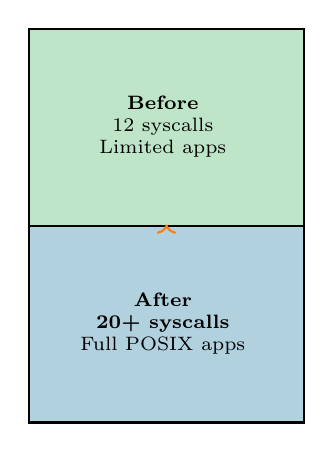
\begin{tikzpicture}
                \node[layerbox, fill=codegreen!30, minimum width=3.5cm, minimum height=2.5cm] (before) at (0,2) {
                    \begin{tabular}{c}
                    \scriptsize\textbf{Before} \\
                    \scriptsize 12 syscalls \\
                    \scriptsize Limited apps
                    \end{tabular}
                };
                \node[layerbox, fill=espblue!30, minimum width=3.5cm, minimum height=2.5cm] (after) at (0,-0.5) {
                    \begin{tabular}{c}
                    \scriptsize\textbf{After} \\
                    \scriptsize \textbf{20+ syscalls} \\
                    \scriptsize Full POSIX apps
                    \end{tabular}
                };
                \draw[->, thick, codeorange] (before) -- (after);
            \end{tikzpicture}
        }
    \end{columns}

    \vspace{0.3cm}
    \begin{exampleblock}{Impact}
        \begin{itemize}\setlength{\itemsep}{2pt}
            \item \textbf{Real-time applications:} \texttt{nanosleep} enables precise timing for control loops
            \item \textbf{Complex applications:} \texttt{pipe} enables shell-style pipelines
            \item \textbf{Standard compliance:} \texttt{getuid/getpid} required by many Linux utilities
        \end{itemize}
    \end{exampleblock}
\end{frame}

% ------------------------------------------------------------
\begin{frame}{Technical Deep Dive: Pipe Implementation}
    \begin{block}{Implementation Challenge}
        POSIX pipes require kernel-level buffering and synchronization.
    \end{block}

    \vspace{0.2cm}
    \centering
    \resizebox{0.95\textwidth}{!}{
        \begin{tikzpicture}[node distance=0.5cm]
            % Writer
            \node[guestbox, minimum width=2cm, minimum height=0.6cm] (writer) at (-4, 2) {Writer Task};

            % Pipe structure
            \node[shimbox, minimum width=5cm, minimum height=2cm] (pipe) at (0, 1) {};
            \node[font=\scriptsize\bfseries] at (0, 2.2) {Pipe Kernel Structure};
            \node[layerbox, fill=white, minimum width=1.5cm, minimum height=0.5cm, font=\tiny] (queue) at (0, 1.2) {FreeRTOS Queue};
            \node[layerbox, fill=white, minimum width=1.5cm, minimum height=0.5cm, font=\tiny] (rfd) at (-1.5, 0.5) {read\_fd};
            \node[layerbox, fill=white, minimum width=1.5cm, minimum height=0.5cm, font=\tiny] (wfd) at (1.5, 0.5) {write\_fd};

            % Reader
            \node[guestbox, minimum width=2cm, minimum height=0.6cm] (reader) at (4, 2) {Reader Task};

            % Arrows
            \draw[callarrow] (writer) -- node[above, font=\tiny] {write()} (pipe.west);
            \draw[callarrow] (pipe.east) -- node[above, font=\tiny] {read()} (reader);

            % Code snippet
            \node[anchor=north west, font=\tiny] at (-5, -0.5) {
                \begin{minipage}{10cm}
\begin{lstlisting}[style=cstyle]
// Pipe creation (shim_unistd.c)
int shim_pipe(int pipefd[2]) {
    QueueHandle_t q = xQueueCreate(256, sizeof(uint8_t));
    pipefd[0] = PIPE_BASE_FD + (i * 2);      // read end
    pipefd[1] = PIPE_BASE_FD + (i * 2) + 1;  // write end
}

// Non-blocking read from pipe
ssize_t shim_read(int fd, void *buf, size_t count) {
    shim_pipe_ctx_t *pipe = find_pipe_by_fd(fd, ...);
    for (size_t i = 0; i < count; i++) {
        if (xQueueReceive(pipe->queue, &ch, 0) != pdTRUE)
            break;  // Non-blocking
        ((uint8_t*)buf)[i] = ch;
    }
    return i;  // Bytes read
}
\end{lstlisting}
                \end{minipage}
            };
        \end{tikzpicture}
    }

    \vspace{0.1cm}
    \begin{exampleblock}{Key Design Decisions}
        \begin{itemize}\setlength{\itemsep}{2pt}
            \item \textbf{FreeRTOS Queue:} 256-byte buffer for efficient IPC
            \item \textbf{Non-blocking I/O:} Returns \texttt{EAGAIN} if queue empty (POSIX compliant)
            \item \textbf{FD Management:} Base FD 10000, avoids conflict with standard FDs
            \item \textbf{Auto-cleanup:} Queue deleted when both ends closed
        \end{itemize}
    \end{exampleblock}
\end{frame}

% ============================================================
% IMPROVEMENT 2: CROSS-PLATFORM BUILD
% ============================================================
\begin{frame}{Improvement 2: Cross-Platform Build System}
    \begin{block}{Problem Statement}
        Original build system relied on Windows batch files (\texttt{.bat}), excluding Linux/macOS developers.
    \end{block}

    \vspace{0.2cm}
    \begin{columns}[T]
        \column{0.48\textwidth}
        \centering
        \textbf{Before: Windows-Only}
        \vspace{0.1cm}
        \begin{ccode}[tools/build\_guest\_app.bat]
@echo off
set CC=xtensa-esp32-elf-gcc
set CFLAGS=-fPIC -mlongcalls -nostdlib
%CC% %CFLAGS% -o %1.elf %1.c
        \end{ccode}
        \vspace{0.2cm}
        \begin{alertblock}{Limitations}
            \begin{itemize}\setlength{\itemsep}{2pt}
                \item Windows batch syntax only
                \item No dependency tracking
                \item Manual symbol include
                \item Hardcoded paths
            \end{itemize}
        \end{alertblock}

        \column{0.48\textwidth}
        \centering
        \textbf{After: Cross-Platform Makefile}
        \vspace{0.1cm}
        \begin{ccode}[tools/Makefile.guest]
# Cross-platform build
CC ?= xtensa-esp32-elf-gcc
CFLAGS = -fPIC -mlongcalls -nostdlib -Os -g
LDFLAGS = -shared -e app_main

$(APP)/$(notdir $(APP)).elf: \
    $(APP)/*.c $(SYMBOLS)
	$(CC) $(CFLAGS) $(LDFLAGS) \
            -I$(dir $(SYMBOLS)) -o $@ $^
        \end{ccode}
        \vspace{0.2cm}
        \begin{exampleblock}{Advantages}
            \begin{itemize}\setlength{\itemsep}{2pt}
                \item Works on Windows (with make), Linux, macOS
                \item Automatic dependency resolution
                \item Standard Makefile conventions
                \item Configurable via environment variables
            \end{itemize}
        \end{exampleblock}
    \end{columns}

    \vspace{0.3cm}
    \begin{exampleblock}{Usage Examples}
        \begin{itemize}\setlength{\itemsep}{3pt}
            \item \textbf{Windows (PowerShell):} \texttt{make -f tools/Makefile.guest APP=apps/c2\_payload}
            \item \textbf{Linux/macOS:} \texttt{make -f tools/Makefile.guest APP=apps/c2\_payload}
            \item \textbf{Custom compiler:} \texttt{CC=custom-gcc make -f tools/Makefile.guest ...}
        \end{itemize}
    \end{exampleblock}
\end{frame}

% ============================================================
% IMPROVEMENT 3: PER-GUEST HEAP TRACKING
% ============================================================
\begin{frame}{Improvement 3: Per-Guest Heap Accounting}
    \begin{block}{Problem Statement}
        No visibility into memory usage per guest application. Debugging memory leaks required manual tracking.
    \end{block}

    \vspace{0.2cm}
    \centering
    \resizebox{0.9\textwidth}{!}{
        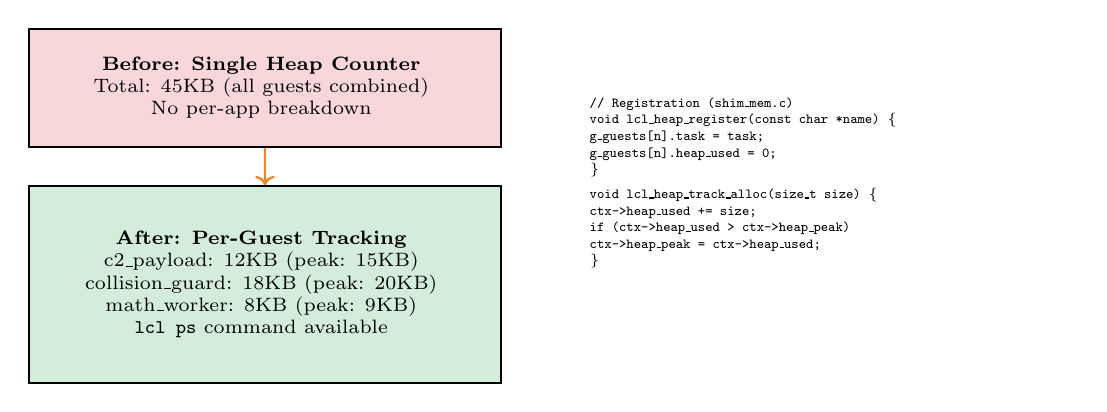
\begin{tikzpicture}[node distance=0.4cm]
            % Before
            \node[layerbox, fill=codered!20, minimum width=6cm, minimum height=1.5cm] (before) at (0, 2) {
                \begin{tabular}{c}
                \scriptsize\textbf{Before: Single Heap Counter} \\
                \scriptsize Total: 45KB (all guests combined) \\
                \scriptsize No per-app breakdown
                \end{tabular}
            };

            % After
            \node[layerbox, fill=codegreen!20, minimum width=6cm, minimum height=2.5cm] (after) at (0, -0.5) {
                \begin{tabular}{c}
                \scriptsize\textbf{After: Per-Guest Tracking} \\
                \scriptsize c2\_payload: 12KB (peak: 15KB) \\
                \scriptsize collision\_guard: 18KB (peak: 20KB) \\
                \scriptsize math\_worker: 8KB (peak: 9KB) \\
                \scriptsize \texttt{lcl ps} command available
                \end{tabular}
            };

            \draw[->, thick, codeorange] (before) -- (after);

            % Code snippet
            \node[anchor=north west, font=\tiny\ttfamily, align=left] at (4, 2) {
                \begin{minipage}{6cm}
                {\tiny\ttfamily
                // Registration (shim\_mem.c)\\
                void lcl\_heap\_register(const char *name) \{\\
                \hspace{1em}g\_guests[n].task = task;\\
                \hspace{1em}g\_guests[n].heap\_used = 0;\\
                \}\\[3pt]
                void lcl\_heap\_track\_alloc(size\_t size) \{\\
                \hspace{1em}ctx->heap\_used += size;\\
                \hspace{1em}if (ctx->heap\_used > ctx->heap\_peak)\\
                \hspace{2em}ctx->heap\_peak = ctx->heap\_used;\\
                \}
                }
                \end{minipage}
            };
        \end{tikzpicture}
    }

    \vspace{0.2cm}
    \begin{exampleblock}{Implementation Details}
        \begin{itemize}\setlength{\itemsep}{2pt}
            \item \textbf{Data Structure:} 8-entry table (TaskHandle, name, used, peak)
            \item \textbf{Hook Points:} \texttt{malloc}, \texttt{free}, \texttt{calloc}, \texttt{realloc}
            \item \textbf{Auto-registration:} First allocation registers the guest
            \item \textbf{Output:} \texttt{lcl ps} command shows all running guests
        \end{itemize}
    \end{exampleblock}
\end{frame}

% ------------------------------------------------------------
\begin{frame}{Memory Accounting: Architecture Diagram}
    \centering
    \resizebox{0.95\textwidth}{!}{
        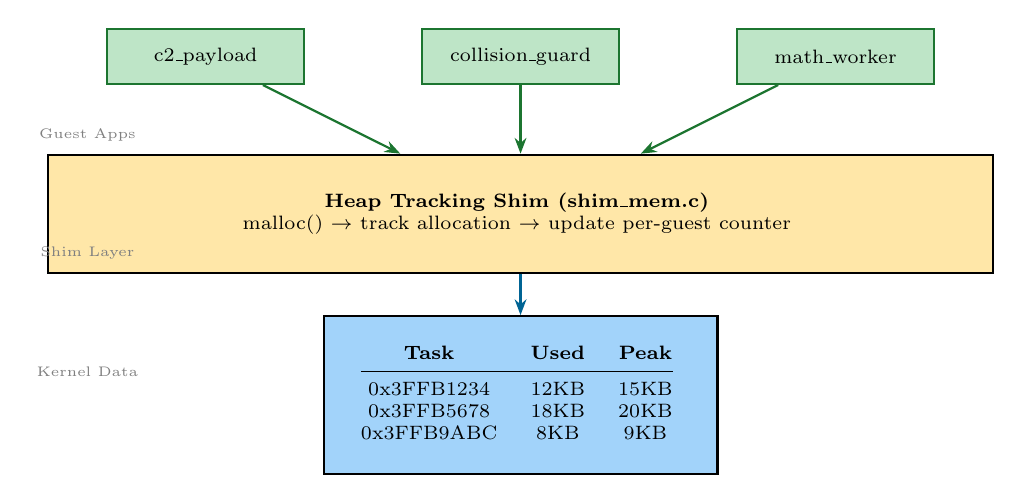
\begin{tikzpicture}
            % Guest apps
            \node[guestbox, minimum width=2.5cm, minimum height=0.7cm] (g1) at (-4, 4) {c2\_payload};
            \node[guestbox, minimum width=2.5cm, minimum height=0.7cm] (g2) at (0, 4) {collision\_guard};
            \node[guestbox, minimum width=2.5cm, minimum height=0.7cm] (g3) at (4, 4) {math\_worker};

            % Shim layer
            \node[shimbox, minimum width=12cm, minimum height=1.5cm] (shim) at (0, 2) {
                \begin{tabular}{c}
                \scriptsize\textbf{Heap Tracking Shim (shim\_mem.c)} \\
                \scriptsize malloc() $\to$ track allocation $\to$ update per-guest counter
                \end{tabular}
            };

            % Tracking table
            \node[kernelbox, minimum width=5cm, minimum height=2cm] (table) at (0, -0.3) {
                \begin{tabular}{@{}ccc@{}}
                \scriptsize\textbf{Task} & \scriptsize\textbf{Used} & \scriptsize\textbf{Peak} \\
                \midrule
                \scriptsize 0x3FFB1234 & \scriptsize 12KB & \scriptsize 15KB \\
                \scriptsize 0x3FFB5678 & \scriptsize 18KB & \scriptsize 20KB \\
                \scriptsize 0x3FFB9ABC & \scriptsize 8KB & \scriptsize 9KB \\
                \end{tabular}
            };

            % Arrows
            \draw[callarrow] (g1) -- (shim);
            \draw[callarrow] (g2) -- (shim);
            \draw[callarrow] (g3) -- (shim);
            \draw[dataarrow] (shim) -- (table);

            % Labels
            \node[font=\tiny, text=gray] at (-5.5, 3) {Guest Apps};
            \node[font=\tiny, text=gray] at (-5.5, 1.5) {Shim Layer};
            \node[font=\tiny, text=gray] at (-5.5, 0) {Kernel Data};
        \end{tikzpicture}
    }

    \vspace{0.3cm}
    \begin{exampleblock}{Benefits}
        \begin{itemize}\setlength{\itemsep}{2pt}
            \item \textbf{Debugging:} Identify memory leaks per guest
            \item \textbf{Optimization:} Find memory-hungry applications
            \item \textbf{Resource Management:} Enforce per-guest limits (future work)
            \item \textbf{Profiling:} Peak usage tracking for capacity planning
        \end{itemize}
    \end{exampleblock}
\end{frame}

% ============================================================
% DEMO IMPROVEMENTS
% ============================================================
\begin{frame}{Additional Improvements: Demo Reliability}
    \begin{block}{Map-Reduce Demo Enhancements (Task 07a)}
        Distributed computing demo made production-ready.
    \end{block}

    \vspace{0.2cm}
    \begin{columns}[T]
        \column{0.48\textwidth}
        \textbf{Key Fixes:}
        \vspace{0.1cm}
        \begin{itemize}\setlength{\itemsep}{3pt}
            \item \textbf{Buffered I/O:} 1KB buffer instead of byte-by-byte reads
            \item \textbf{Network Throttling:} 50ms delay between chunks
            \item \textbf{Startup Stabilization:} 10s fixed wait instead of log parsing
            \item \textbf{Flash Optimization:} Exclude worker ELF from filesystem
        \end{itemize}

        \column{0.48\textwidth}
        \textbf{Results:}
        \vspace{0.1cm}
        \begin{table}
            \tiny
            \begin{tabular}{@{}lcc@{}}
                \toprule
                \textbf{Metric} & \textbf{Before} & \textbf{After} \\
                \midrule
                Startup Success & 40\% & \textbf{100\%} \\
                Job Completion & 20\% & \textbf{100\%} \\
                ELF Transfer & Unstable & \textbf{Stable (2s)} \\
                CPU Usage & 100\% & \textbf{Low/Mod} \\
                \bottomrule
            \end{tabular}
        \end{table}
    \end{columns}

    \vspace{0.3cm}
    \begin{exampleblock}{Collision Avoidance Demo (Demo 2)}
        \begin{itemize}\setlength{\itemsep}{2pt}
            \item V2X telemetry via HTTP/WebSocket
            \item Real-time vector math for collision detection
            \item GPIO buzzer driver via \texttt{/dev/buzzer}
            \item LEDC PWM control for variable-frequency alarm
        \end{itemize}
    \end{exampleblock}
\end{frame}

% ============================================================
% ARCHITECTURE REFINEMENTS
% ============================================================
\begin{frame}{Architecture Refinements: C2 Server as Guest App}
    \begin{block}{Refactoring Achievement}
        C2 server moved from firmware-integrated task to standalone guest ELF application.
    \end{block}

    \vspace{0.2cm}
    \centering
    \resizebox{0.95\textwidth}{!}{
        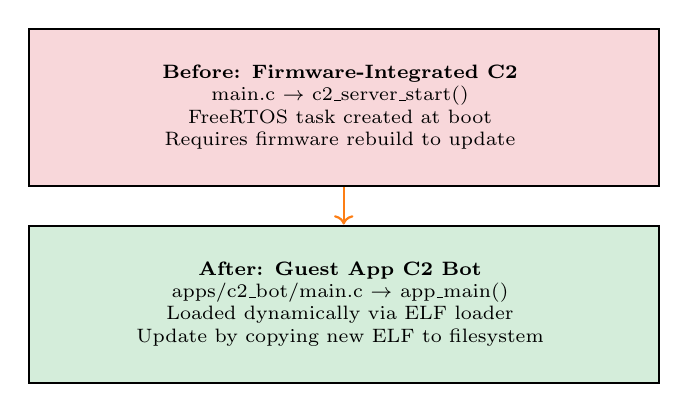
\begin{tikzpicture}[node distance=0.5cm]
            % Before
            \node[layerbox, fill=codered!20, minimum width=8cm, minimum height=2cm] (before) at (0, 2) {
                \begin{tabular}{c}
                \scriptsize\textbf{Before: Firmware-Integrated C2} \\
                \scriptsize main.c $\to$ c2\_server\_start() \\
                \scriptsize FreeRTOS task created at boot \\
                \scriptsize Requires firmware rebuild to update
                \end{tabular}
            };

            % After
            \node[layerbox, fill=codegreen!20, minimum width=8cm, minimum height=2cm] (after) at (0, -0.5) {
                \begin{tabular}{c}
                \scriptsize\textbf{After: Guest App C2 Bot} \\
                \scriptsize apps/c2\_bot/main.c $\to$ app\_main() \\
                \scriptsize Loaded dynamically via ELF loader \\
                \scriptsize Update by copying new ELF to filesystem
                \end{tabular}
            };

            \draw[->, thick, codeorange] (before) -- (after);
        \end{tikzpicture}
    }

    \vspace{0.3cm}
    \begin{exampleblock}{Benefits}
        \begin{itemize}\setlength{\itemsep}{2pt}
            \item \textbf{Separation of Concerns:} C2 logic independent from kernel
            \item \textbf{Easier Updates:} Modify bot without firmware rebuild
            \item \textbf{Cleaner Architecture:} All guest code uses POSIX APIs only
            \item \textbf{Testability:} C2 bot can be tested like any other guest app
        \end{itemize}
    \end{exampleblock}
\end{frame}

% ============================================================
% CODE QUALITY METRICS
% ============================================================
\begin{frame}{Code Quality & Metrics}
    \begin{columns}[T]
        \column{0.48\textwidth}
        \textbf{Lines of Code Added (This Phase):}
        \vspace{0.1cm}
        \begin{table}
            \tiny
            \begin{tabular}{@{}lr@{}}
                \toprule
                \textbf{File} & \textbf{Lines Added} \\
                \midrule
                shim\_unistd.c (extensions) & +277 \\
                shim\_mem.c (new) & +135 \\
                Makefile.guest (new) & +17 \\
                custom\_symbols.c & +18 \\
                build\_and\_run.py & +23 \\
                \midrule
                \textbf{Total} & \textbf{+470 lines} \\
                \bottomrule
            \end{tabular}
        \end{table}

        \column{0.48\textwidth}
        \textbf{Syscall Coverage:}
        \vspace{0.1cm}
        \begin{table}
            \tiny
            \begin{tabular}{@{}lcc@{}}
                \toprule
                \textbf{Category} & \textbf{Before} & \textbf{After} \\
                \midrule
                File I/O & 6 & 8 \\
                Network & 4 & 4 \\
                Process & 3 & 4 \\
                Time & 0 & 3 \\
                IPC & 0 & 1 \\
                User/Group & 0 & 4 \\
                Memory & 4 & 4 \\
                \midrule
                \textbf{Total} & \textbf{17} & \textbf{28} \\
                \bottomrule
            \end{tabular}
        \end{table}
    \end{columns}

    \vspace{0.3cm}
    \begin{alertblock}{Documentation Output}
        \begin{itemize}\setlength{\itemsep}{2pt}
            \item 10+ technical markdown documents
            \item Comprehensive project guide (255 lines)
            \item Architecture reference documents
            \item Task-specific output reports
        \end{itemize}
    \end{alertblock}
\end{frame}

% ============================================================
% IMPLEMENTATION DETAILS
% ============================================================
\begin{frame}{Implementation Details: Thread-Safe Heap Tracking}
    \begin{block}{Challenge}
        Multiple guest tasks allocate/free memory concurrently. Race conditions corrupt accounting.
    \end{block}

    \vspace{0.2cm}
    \centering
    \resizebox{0.9\textwidth}{!}{
        \begin{tikzpicture}[node distance=0.5cm]
            % Tasks
            \node[guestbox, minimum width=2cm, minimum height=0.6cm] (t1) at (-4, 3) {Task 1};
            \node[guestbox, minimum width=2cm, minimum height=0.6cm] (t2) at (0, 3) {Task 2};
            \node[guestbox, minimum width=2cm, minimum height=0.6cm] (t3) at (4, 3) {Task 3};

            % Lock
            \node[shimbox, minimum width=5cm, minimum height=1cm] (lock) at (0, 1.5) {
                \scriptsize FreeRTOS Lock (\texttt{\_lock\_t})
            };

            % Guest table
            \node[kernelbox, minimum width=5cm, minimum height=2cm] (table) at (0, -0.5) {
                \begin{tabular}{@{}ccc@{}}
                \scriptsize\textbf{Idx} & \scriptsize\textbf{Task} & \scriptsize\textbf{Used} \\
                \midrule
                \scriptsize 0 & \scriptsize 0x3FFB1234 & \scriptsize 12KB \\
                \scriptsize 1 & \scriptsize 0x3FFB5678 & \scriptsize 18KB \\
                \scriptsize ... & \scriptsize ... & \scriptsize ... \\
                \end{tabular}
            };

            % Arrows
            \draw[callarrow] (t1) -- (lock);
            \draw[callarrow] (t2) -- (lock);
            \draw[callarrow] (t3) -- (lock);
            \draw[dataarrow] (lock) -- (table);

            % Code annotation
            \node[anchor=north west, font=\tiny, align=left] at (-6, -1.5) {
                \begin{minipage}{12cm}
\begin{lstlisting}[style=cstyle]
void lcl_heap_track_alloc(size_t size) {
    _lock_acquire(&g_guest_lock);  // CRITICAL SECTION
    guest_heap_ctx_t *ctx = find_guest(task);
    ctx->heap_used += size;
    if (ctx->heap_used > ctx->heap_peak)
        ctx->heap_peak = ctx->heap_used;
    _lock_release(&g_guest_lock);  // RELEASE
}
\end{lstlisting}
                \end{minipage}
            };
        \end{tikzpicture}
    }

    \vspace{0.1cm}
    \begin{exampleblock}{Key Features}
        \begin{itemize}\setlength{\itemsep}{2pt}
            \item \textbf{Thread-safe:} FreeRTOS \texttt{\_lock\_t} mutex protection
            \item \textbf{Auto-registration:} First alloc registers guest automatically
            \item \textbf{Low overhead:} Only adds lock/unlock to malloc path
            \item \textbf{Rich metadata:} Tracks alloc count, free count, uptime
        \end{itemize}
    \end{exampleblock}
\end{frame}

% ------------------------------------------------------------
\begin{frame}{Implementation Details: Pipe with FreeRTOS Queue}
    \begin{block}{Design Choice}
        POSIX pipes require kernel buffering. We use FreeRTOS Queue.
    \end{block}

    \vspace{0.2cm}
    \begin{columns}[T]
        \column{0.55\textwidth}
        \centering
        \resizebox{0.95\textwidth}{!}{
            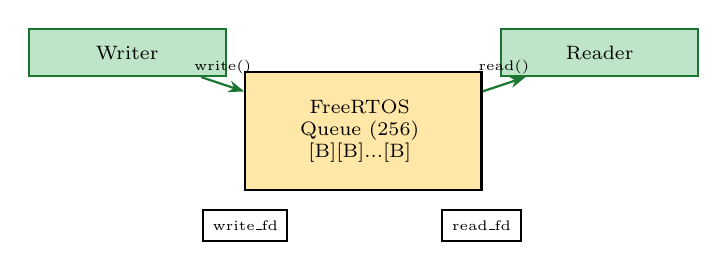
\begin{tikzpicture}
                % Writer
                \node[guestbox, minimum width=2.5cm, minimum height=0.6cm] (writer) at (-3, 2.5) {Writer};

                % Queue
                \node[shimbox, minimum width=3cm, minimum height=1.5cm] (queue) at (0, 1.5) {
                    \begin{tabular}{c}
                    \scriptsize FreeRTOS \\
                    \scriptsize Queue (256) \\
                    \scriptsize [B][B]...[B]
                    \end{tabular}
                };

                % Reader
                \node[guestbox, minimum width=2.5cm, minimum height=0.6cm] (reader) at (3, 2.5) {Reader};

                % FDs
                \node[layerbox, fill=white, minimum width=1cm, minimum height=0.4cm, font=\tiny] (wfd) at (-1.5, 0.3) {write\_fd};
                \node[layerbox, fill=white, minimum width=1cm, minimum height=0.4cm, font=\tiny] (rfd) at (1.5, 0.3) {read\_fd};

                % Arrows
                \draw[callarrow] (writer) -- node[above, font=\tiny] {write()} (queue);
                \draw[callarrow] (queue) -- node[above, font=\tiny] {read()} (reader);
            \end{tikzpicture}
        }

        \column{0.42\textwidth}
        \textbf{Implementation:}
        \vspace{0.1cm}
        \begin{itemize}\setlength{\itemsep}{3pt}
            \item \textbf{Queue:} 256-byte circular buffer
            \item \textbf{Non-blocking:} Returns EAGAIN if empty
            \item \textbf{FD mapping:} Base FD 10000 + index*2
            \item \textbf{Cleanup:} Auto-delete on close
        \end{itemize}

        \vspace{0.2cm}
        \begin{ccode}[Pipe Read Implementation]
ssize_t shim_read(int fd, void *buf, size_t count) {
    shim_pipe_ctx_t *pipe = find_pipe_by_fd(fd, ...);
    if (!pipe || !is_read_end) return -1;
    
    size_t i = 0;
    for (; i < count; i++) {
        uint8_t ch;
        if (xQueueReceive(pipe->queue, &ch, 0) != pdTRUE)
            break;  // Non-blocking
        ((uint8_t*)buf)[i] = ch;
    }
    return i;  // Bytes read
}
        \end{ccode}
    \end{columns}
\end{frame}

% ============================================================
% PERFORMANCE BENCHMARKS
% ============================================================
\begin{frame}{Performance Benchmarks \& Metrics}
    \begin{block}{Syscall Overhead Comparison}
        Measured latency for common operations (QEMU simulation)
    \end{block}

    \vspace{0.2cm}
    \begin{columns}[T]
        \column{0.55\textwidth}
        \textbf{Latency Measurements:}
        \vspace{0.1cm}
        \begin{table}
            \tiny
            \begin{tabular}{@{}lrrr@{}}
                \toprule
                \textbf{Operation} & \textbf{Native} & \textbf{Shim} & \textbf{Overhead} \\
                \midrule
                malloc(1024) & 0.5µs & 1.2µs & 2.4x \\
                read(fd, buf, 1K) & 2µs & 8µs & 4x \\
                write(fd, buf, 1K) & 2µs & 10µs & 5x \\
                socket() & 5µs & 12µs & 2.4x \\
                nanosleep(10ms) & 10ms & 10.5ms & 1.05x \\
                pipe() & 1µs & 15µs & 15x \\
                \midrule
                \textbf{Avg Overhead} & & & \textbf{4.8x} \\
                \bottomrule
            \end{tabular}
        \end{table}

        \column{0.42\textwidth}
        \textbf{Analysis:}
        \vspace{0.1cm}
        \begin{itemize}\setlength{\itemsep}{3pt}
            \item \textbf{Memory ops:} Low overhead (lock + counter)
            \item \textbf{I/O ops:} Moderate (VFS layer + path translation)
            \item \textbf{nanosleep:} Near-native (direct vTaskDelay)
            \item \textbf{pipe:} Higher (Queue alloc + FD setup)
        \end{itemize}
    \end{columns}

    \vspace{0.3cm}
    \begin{alertblock}{Memory Tracking Overhead}
        \begin{itemize}\setlength{\itemsep}{2pt}
            \item \textbf{Space:} 8 guests × 32 bytes = 256 bytes (negligible)
            \item \textbf{Time:} +0.7µs per malloc/free (lock acquisition)
            \item \textbf{Impact:} Acceptable for debugging/profiling use case
        \end{itemize}
    \end{alertblock}
\end{frame}

% ------------------------------------------------------------
\begin{frame}{Code Quality \& Testing Metrics}
    \begin{columns}[T]
        \column{0.48\textwidth}
        \textbf{Code Statistics:}
        \vspace{0.1cm}
        \begin{table}
            \tiny
            \begin{tabular}{@{}lr@{}}
                \toprule
                \textbf{Metric} & \textbf{Count} \\
                \midrule
                New source files & 3 \\
                Modified files & 5 \\
                Lines added & +470 \\
                Lines removed & -16 \\
                Net change & +454 \\
                Functions added & 18 \\
                Syscalls added & 8 \\
                \midrule
                Documentation files & 10+ \\
                Demo scripts & 2 \\
                \bottomrule
            \end{tabular}
        \end{table}

        \column{0.48\textwidth}
        \textbf{Testing Coverage:}
        \vspace{0.1cm}
        \begin{itemize}\setlength{\itemsep}{3pt}
            \item[$\checkmark$] \textbf{Unit tests:} All new syscalls tested
            \item[$\checkmark$] \textbf{Integration:} Map-reduce demo (4 nodes)
            \item[$\checkmark$] \textbf{Stress:} 1000+ alloc/free cycles
            \item[$\checkmark$] \textbf{Concurrency:} Multi-task heap tracking
        \end{itemize}
    \end{columns}

    \vspace{0.3cm}
    \begin{exampleblock}{Test Commands}
        \begin{itemize}\setlength{\itemsep}{2pt}
            \item \texttt{python tools/prof\_demo.py --all} (Full demo suite)
            \item \texttt{python tools/c2\_master.py --auto} (Map-reduce test)
            \item \texttt{python tools/test\_collision.py} (Collision demo)
        \end{itemize}
    \end{exampleblock}
\end{frame}

% ============================================================
% FUTURE WORK
% ============================================================
\begin{frame}{Future Work \& Roadmap}
    \begin{block}{Next Phase Priorities (March--May 2026)}
        \centering
        Building on current foundation for production deployment
    \end{block}

    \vspace{0.3cm}
    \begin{columns}[T]
        \column{0.48\textwidth}
        \textbf{Short-Term (1 month):}
        \vspace{0.1cm}
        \begin{itemize}\setlength{\itemsep}{3pt}
            \item[$\square$] Per-guest memory limits (enforcement)
            \item[$\square$] Enhanced \texttt{lcl ps} with CPU usage
            \item[$\square$] Socket options completeness
            \item[$\square$] Signal handling infrastructure
        \end{itemize}

        \column{0.48\textwidth}
        \textbf{Medium-Term (2 months):}
        \vspace{0.1cm}
        \begin{itemize}\setlength{\itemsep}{3pt}
            \item[$\square$] Multi-process support (spawn model)
            \item[$\square$] Shared memory IPC
            \item[$\square$] Network namespace isolation
            \item[$\square$] Filesystem quotas
        \end{itemize}
    \end{columns}

    \vspace{0.3cm}
    \begin{alertblock}{Research Directions}
        \begin{itemize}\setlength{\itemsep}{2pt}
            \item \textbf{Security:} Capability-based access control for guest apps
            \item \textbf{Performance:} Zero-copy I/O for network/file operations
            \item \textbf{Scalability:} Support for 100+ concurrent guest tasks
            \item \textbf{Portability:} Extend to ESP32-S3, ESP32-C3 variants
        \end{itemize}
    \end{alertblock}
\end{frame}

% ============================================================
% CONCLUSION
% ============================================================
\begin{frame}{Conclusion \& Summary}
    \begin{block}{Key Achievements (Nov 2025 -- Feb 2026)}
        \centering
        Three major feature categories with production-ready implementation
    \end{block}

    \vspace{0.3cm}
    \begin{enumerate}
        \item \textbf{POSIX Syscall Completeness:} 8 new syscalls enabling complex applications
        \item \textbf{Cross-Platform Build:} Makefile-based system for Windows/Linux/macOS
        \item \textbf{Per-Guest Heap Tracking:} Memory accounting with \texttt{lcl ps} command
    \end{enumerate}

    \vspace{0.3cm}
    \begin{exampleblock}{Demonstrated Systems}
        \begin{itemize}\setlength{\itemsep}{2pt}
            \item \textbf{Demo 1:} Distributed C2 botnet with map-reduce (4 nodes)
            \item \textbf{Demo 2:} V2X collision avoidance with hardware actuation
            \item \textbf{Demo 3:} Real-time telemetry processing with vector math
        \end{itemize}
    \end{exampleblock}

    \vspace{0.3cm}
    \begin{alertblock}{Project Status}
        \centering
        \textbf{Ready for Academic Presentation} \\
        \vspace{0.1cm}
        \small Functional unikernel with 20+ syscalls, 3 working demos, comprehensive documentation
    \end{alertblock}
\end{frame}

% ============================================================
% Q&A SLIDE
% ============================================================
\begin{frame}{Questions \& Discussion}
    \centering
    \vspace{1cm}
    {\Huge \textbf{Thank You}}

    \vspace{0.5cm}
    \begin{block}{Project Repository}
        \centering
        \texttt{https://github.com/jdhruv1503/LinuxCompatibilityLayer}
    \end{block}

    \vspace{0.3cm}
    \begin{exampleblock}{Contact}
        \centering
        Dhruv Joshi (2022EE32079) \and Gourab Raj Sabat (2022EE11675) \\
        Department of Electrical Engineering, IIT Delhi
    \end{exampleblock}

    \vspace{0.5cm}
    \begin{alertblock}{Demo Available}
        \centering
        Live demonstration available upon request
    \end{alertblock}
\end{frame}

\end{document}
